
Jokaisella hypyllä kannattaa mahdollisuuksien mukaan harjoitella varjon käyttöä, kuten esimerkiksi tarkkuusniksiä ja erilaisia käännöksiä. Kun lähdet hyppäämään sinulle uuden tyyppisellä tai kokoisella varjolla, tee ensin ainakin harjoitushypyt 1-4 ja ala vasta sitten käyttämään varjoa muilla hypyillä. Näin saat ensin harjoitusta varjon lentämisestä ja laskeutumisesta.  


\textbf{Huom!} Varjon pitää aina olla lentokuntoinen viimeistään 600 metrin korkeudessa. Myös puolijarrujen täytyy olla tuolloin avattuina! 

\section{ Hyppy 1 }
\label{kuvunkasittelyharjoitukset-hyppy-1}


Tarkoituksena on oppia tuntemaan oman varjon ominaisuudet ja oppia tekemään loppuveto. Hyppykorkeus vähintään 2000 m, 8-10 sekunnin vapaa. Kokeile ohjaamista ja fleeraamista takakantohihnoista ennen jarrujen avaamista. Näin voit harjoitella nopeaa väistämistä heti avauksen jälkeen. 


Avaa puolijarrut ja harjoittele loppuvetoa täysiliidosta. Muista terävä alkuveto ja sen jälkeen jarrutuksen lisääminen vähitellen. Valmistaudu alastulokuvioon huomioiden porrastukset. Huomioi mahdollisen kuvaajan sijainti äläkä lennä suoraan kohti. Tee oikeaoppinen loppuveto täydestä liidosta. 

\section{ Hyppy 2 }
\label{kuvunkasittelyharjoitukset-hyppy-2}


Hyppykorkeus vähintään 2000 m, 8-10 sekunnin vapaa. Avaa puolijarrut. Kokeile käännöksiä eri lentotiloissa (puolijarrutus, täysijarrutus) molempiin suuntiin. Kokeile käännöksiä etu- ja takakantohihnoista molempiin suuntiin.  


Kokeile 360 asteen käännöstä ja pysäytystä ennalta päättämääsi suuntaan. Huomioi, kuinka paljon aikaisemmin käännös täytyy lopettaa, että pysäytys tapahtuu valitsemaasi suuntaan. Huomioi myös, kuinka suuri vastaliike täytyy tehdä, että käännös pysähtyy. 


Kokeile samaa, mutta 90 asteen käännöksellä. Huomioi edellämainitut asiat. Kokeile loppuvetoa ja loppuvedon aikana myös 90 asteen käännöstä. Seuraa korkeuden menetystä käännösten aikana. 


Valmistaudu alastulokuvioon huomioiden porrastukset ja kuvaaja. Tee oikeaoppinen loppuveto täydestä liidosta. 

\section{ Hyppy 3 }
\label{kuvunkasittelyharjoitukset-hyppy-3}


Exit ja vapaa sama kuin edellisissä hypyissä. Harjoittele loppuvetoa puolijarrutustilasta. Huomaat, että tarvittava veto on terävämpi. Koita myös loppuvetoa takimmaisista kantohihnoista. Valmistaudu alastulokuvioon huomioiden porrastukset ja kuvaaja. Finaali ja loppuveto puolijarruilta. 

\section{ Hyppy 4 }
\label{kuvunkasittelyharjoitukset-hyppy-4}


Tarkoitus on oppia tarkkuusniksi ja oman varjon optimaalinen jarrujen tai takakantohihnojen asento matkalennossa. Hyppykorkeus yli 2000 m, mielellään mahdollisimman korkealla, 8–10 sekunnin vapaa, uloshypyt viiden sekunnin välein ja 3-5 hyppääjää samalla linjalla. Uloshyppypaikka 2–4 kertaa kauempana kuin normaalisti. Huomioi mahdolliset varalaskupaikat suunnitellessasi UH-paikkaa. 


Kokoontukaa ennen jarrujen/kantohihnojen vaikutuksen testaamista puljalentoa varten. Lentäkää matkalentoa ryhmässä. Vertaile omaa lentämistä vierustovereihin nähden, kulkeeko ja vajoaako varjosi nopeammin vai hitaammin kuin muilla, kun lisäät jarruja tai vedät takakantohihnoista. Harjoittele tarkkuusniksin käyttöä ja etsi varjostasi jarrujen ja takakantohihnojen paras asento matkalennon suhteen. 


Valmistaudu alastulokuvioon huomioiden porrastukset ja kuvaaja. Finaali ja loppuveto puolijarruilla. 

\section{ Hyppy 5 }
\label{kuvunkasittelyharjoitukset-hyppy-5}


Vaihtoehtoina esimerkiksi:  

\begin{itemize}
\item  Toisen hyppääjän kanssa ennalta sovitusti seuraa johtajaa -leikki. Liikesarja on syytä sopia maassa ennen hyppyä! Esimerkiksi kaksi kertaa vasen 360°, oikea 360°, pysäytys, hidaslentoa jarruilla ja sitten samat käännökset hidaslennossa. Johtaja varmistaa, että perässä pysytään. Tarvittaessa liikesarja keskeytetään ja odotetaan.  
\item  Tarkkuusniksin harjoittelua. Kokeile myös korkealla ensin vauhdinotto etukantohihnoista ja siitä loppuveto. Testaa myös korkealla 90° käännöstä loppuvedon aikana. 
\end{itemize}
\section{ Laskeutumisen kuvaamisesta }
\label{kuvunkasittelyharjoitukset-laskeutumisen-kuvaamisesta}


Kuvaaminen kuuluu olennaisena osana hyppyjen arviointiin. Virheet tapahtuvat usein lyhyessä ajassa, ja siksi videolta hidastettuna, jopa kuva kuvalta katsottuna, ne tulevat parhaiten esiin. 


Sovi ennen kuvaamista hyppääjien kanssa oma paikkasi maalialueella, laskeutumissuunta, sekä mihin kohtaan hyppääjän tulisi pysähtyä. Sovi myös porrastuksista, etteivät kaikki tule yhtä aikaa laskuun. Jos pokalla on muita hyppääjiä, vältetään kuvattavien hyppääjien laskeutumista samaan laskeutumispaikkaan heidän kanssaan. 


Suunnittele kuvauspaikka niin, että aurinko ei ole hyppääjän takana hänen ollessaan finaalissa. Paras auringon paikka on kuvaajan takana. Mikäli aloitat kuvaamisen hyppääjän ollessa myötätuuliosalla, voi auringon valo aiheuttaa hetkellisen sokeutumisen. Vältä tummaa taustaa, esimerkiksi havupuumetsää. Hyppääjän korkeuden laskiessa latvuston korkeuden alle kirkas taivas ja tumma tausta voivat aiheuttaa sen, että kamera ei reagoi tarpeeksi nopeasti valon muutokseen ja kuvasta tulee tumma. Myös hyppääjän käsien liikkeitä on tällöin vaikeaa arvioida. 


Kuvatessasi laskeutuvaa hyppääjää, sijoita hyppääjä kuvaruutuun niin, että hän peittää pystysuunnassa kaksi kolmasosaa ja että hyppääjän edessä sekä alla on tyhjää tilaa. 


\begin{Figure}\centering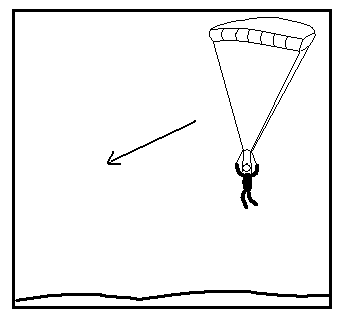
\includegraphics[width=0.7\textwidth]{Laskeutumisen-kuvaus.png}\captionof{figure}{Kuvaruudun pitäisi näyttää tältä laskeutumista kuvattaessa.}\end{Figure} 


Pyri pitämään maa näkyvissä vertailukohteena loppuvedon aloittamiskorkeuden arviointia varten. Vältä kaukaa kuvaamista ja zoomin edestakaista käyttöä. Kuvaa samalta (maanpinnan) tasolta kuin mihin hyppääjät laskeutuvat. 


Kuvaajan tulisi sijoittua niin, että nauhalla näkyy koko ajan hyppääjän molemmat kädet, kuvun takahelma ja hyppääjän eteenpäin menevä liike loppuvedon aikana. Sijoitu niin, että hyppääjän finaali on noin 45 asteen kulmassa kohti kuvaajaa ja hyppääjän vauhti loppuu ennen kuvaajan tasolle saapumista. Suoraan edestä kuvattaessa eteenpäin menevää liikettä ei näy ja sivulta kuvattaessa toinen käsi jää hyppääjän vartalon taakse. Takaa sivulta kuvattuna em. liikkeet näkyvät hyvin. 


Hyppyä videolta arvioidessasi keskitä huomiosi seuraaviin seikkoihin. 

\begin{enumerate}[label=\bfseries \arabic*)]
\item  Päähän/kypärään, josta näet onko hyppääjä siirtynyt vaakalentoon. 
\item  Käsiin, joista näet hyppääjän tekemät ohjausliikkeet ja mahdolliset virheet. 
\item  Kuvun takahelmaan, josta näet siirtyykö koko kupu vaakalentoon. Takahelmasta näet myös kohtien 1 ja 2 asiat. 
\end{enumerate}

Keskity vain kuvaamiseen. Älä yritä arvioida laskeutumisia. Ne arvioidaan jälkikäteen videolta. 

